\chapter{Hydrodynamical simulations with PLUTO} \label{chapter2}
%\doublespacing
%% TBD Fix table with new values of n_e (done)






For my simulations, I use the publicly available PLUTO code \citep{mignone07} to produce two dimensional axisymmetric and three dimensional hydrodynamic models of the jet-ICM interaction in Hydra A. 
PLUTO is a highly efficient code for the study of supersonic, astrophysical jets because it uses a high resolution shock capturing Godunov-type scheme. Hence, I use this code to study the structures of the Hydra A northern jet, including two bright knots (which I assume to be reconfinement shocks), curvature of the jet, the jet-plume transition and the interaction of the radio source with the cluster atmosphere. The detail of the models are given in chapters~\ref{chapter5} and \ref{chapter8}.

PLUTO is a finite volume hydrodynamic code for computational astrophysics written in C. This software is modular and highly user friendly. It provides an interactive interface (written in python) to select problem dependent physics module and algorithms. Using the message passing interface (MPI) this code can run in multiple processors in parallel. The scalability of the PLUTO code based on one of my three-dimensional jet-ICM interaction models (run A of chapter~\ref{chapter8}) is described in this chapter (see \S~\ref{s:pt}). I ran my models of Hydra A jets with a maximum of 2048 processors using the National Computing Infrastructure supercomputers VAYU and RAIJIN at ANU. 

%Utilysing my three dimensional jet model, I perform a scaling test for the PLUTO code with a minimum 64 cpus to a maximum 2048 cpus (see \S~\ref{s:pt}).


%In the pressure image of the inner 6~kpc (Fig.~\ref{rsk}) of one of my two dimensional axisymmetric models . 

%The structure of the PLUTO is modular which makes it very flexible

%%%%%%%%%%%%%%%%%%%%%%%%%%%%%%%%%%%%%%
% 		RELATIVISTIC HYDRODYNAMIC EQUATIONS
%%%%%%%%%%%%%%%%%%%%%%%%%%%%%%%%%%%%%%
\section{Relativistic hydrodynamic equations}
Since my models involve relativistic velocities, I use the relativistic hydrodynamic (RHD) module available in PLUTO to solve the relativistic fluid equations. 

Let $\rho$ be the proper density, $p$ the pressure, $\textbf{v} =( v_1, v_2, v_3)$ the velocity, $D$ the laboratory density, $\textbf{m} = (m_1, m_2, m_3)$ the momentum, $E$ the total energy. The conservative quantities  $\textbf{U} = (D, \textbf{m}, E)$ is related to the conservative quantities $\textbf{V} = (\rho, p, \textbf{v})$by:
\begin{eqnarray}
D = \rho \Gamma, \nonumber \\  
\textbf{m} = \rho h \Gamma^2 \textbf{v}, \\
E = \rho h \Gamma^2 -p \nonumber,
\end{eqnarray}
where $\Gamma = 1/\sqrt{1 - v^2}$ is the Lorentz factor (when the speed of light is 1), and $h = (E+p)/\rho$ is the specific enthalpy.

The relativistic Euler equations in conservative form are  \citep{pluto12}:
\begin{eqnarray}
\frac{\partial D}{\partial t} +  \nabla \cdot (D\textbf{v})= 0  \label{eq:d},\\
\frac{\partial \textbf{m}}{\partial t} + \nabla \cdot (\textbf{m}\textbf{v} + p\textbf{I}) = D\textbf{g},  \label{eq:m}\\
\frac{\partial E}{\partial t} + \nabla \cdot \textbf{m}  = \textbf{m} \cdot \textbf{g}. \label{eq:e}
\end{eqnarray}

In these equations the first term represents time derivative of the conservative variables, the second term represents the divergence of the fluxes $\textbf{F} =(D \textbf{v}, \textbf{mv}+ p\textbf{I}, \textbf{m})$ and the right hand side represents the source term \textbf{S}, arising from gravitation; $\textbf{g}$ is the  gravitational acceleration vector. 

%In terms of primitive variables $\textbf{V}=(p, \textbf{v}, p)$, Eqns.~\ref{eq:d}--\ref{eq:e} are: 
%\begin{eqnarray}
%\frac{\partial \rho}{\partial t}+ \textbf{v}.\nabla \rho- \frac{1}{c_s^2 h} . \nabla p = \frac{1}{c_s^2 h} \frac{\partial p}{\partial t},        \nonumber \\
%\frac{\partial  \textbf{v}}{\partial t}+ \textbf{v}.\nabla  \textbf{v} + \frac{1}{\rho h \Gamma^2}\nabla p = - \frac{v}{\rho h \Gamma^2} \frac{\partial p}{\partial t}+\textbf{g}, 			\label{eq:Eeq_p}		\\
%\frac{\partial p}{\partial t} + \frac{1}{1-v^2c_s^2}[ c_s^2 \rho h \nabla . \textbf{v} + (1-c_s^2) \textbf{v} . \nabla p ]= 	0,	\nonumber 
%\end{eqnarray}
%where $c_s = \sqrt{\gamma p/\rho}$ is the sound speed.

An additional relation between the thermodynamic quantities, the equation of state (EOS), is also available: 
\begin{equation}
h = h(p, \rho).
\label{eq:eos}
\end{equation}
In my models I use the \citet{taub1948a} equation of state, a quadratic approximation to the exact Synge--J\"{u}ttner relativistic perfect gas equation of state \citep{juttner1911a,synge1957a}, which yields $\gamma\rightarrow5/3$ in the low temperature limit, and $\gamma\rightarrow4/3$ in the high temperature limit. For the Taub equation of state the enthalpy equation becomes:
\begin{equation}
h = \frac{5}{2}\frac{p}{\rho} + \sqrt{\frac{9}{4} \left (\frac{p}{\rho} \right )^2 + 1}.
\label{eq:enth}
\end{equation}

To obtain the temporal evolution of the states at each cell, the Eqns.~\ref{eq:d}--\ref{eq:e} together with the equation of state (Eq.~\ref{eq:enth}) need to be solved numerically. Below, I briefly describe how the numerical code PLUTO solves these special relativistic fluid equations.




%
%Let $D$ be the laboratory density, $\textbf{m}$ the momentum density, $\textbf{v}$ the velocity, $E$ the total energy, $p$ the thermal pressure, and $\textbf{g}$ the gravitational acceleration, then the relativistic Euler equations in conservative form \citep{pluto12}:
%%\begin{equation}
%%\frac{\partial}{\partial t}
%% \begin{pmatrix}
%%D \\
%%\textbf{m}\\
%%E
%% \end{pmatrix}
%% +
%% \nabla . 
%%  \begin{pmatrix}
%%D\textbf{v} \\
%%\textbf{m}\textbf{v} + p\textbf{I}\\
%%\textbf{m} 
%%\end{pmatrix}
%%=
%%  \begin{pmatrix}
%%0 \\
%%D\textbf{g}\\
%%\textbf{m}. \textbf{g}
%%\end{pmatrix}
%%\label{eq:Eeq}
%%\end{equation}
%
%\begin{eqnarray}
%\frac{\partial D}{\partial t} +  \nabla \cdot (D\textbf{v})= 0  \label{eq:d}\\
%\frac{\partial \textbf{m}}{\partial t} + \nabla \cdot (\textbf{m}\textbf{v}) + p\textbf{I} = D\textbf{g}  \label{eq:m}\\
%\frac{\partial E}{\partial t} + \nabla \cdot \textbf{m}  = \textbf{m} \cdot \textbf{g} \label{eq:e}
%\end{eqnarray}
%
%In these equations the first term represents derivative of the conservative variables $\textbf{U}=(D,\textbf{m}, E)$, %which are the required quatities at each cell 
%the second term represents the divergence of the fluxes $\textbf{F} = (D \textbf{v}, \textbf{mv}+ p\textbf{I}, \textbf{m})$ and the right hand side represents the source term \textbf{S}, arising from gravitation. 
%
%
%
%In terms of primitive variables $\textbf{V}=(p, \textbf{v}, p)$, Eqns.~\ref{eq:d}--\ref{eq:e} are: 
%\begin{eqnarray}
%\frac{\partial \rho}{\partial t}+ \textbf{v}.\nabla \rho- \frac{1}{c_s^2 h} . \nabla p = \frac{1}{c_s^2 h} \frac{\partial p}{\partial t}        \nonumber \\
%\frac{\partial  \textbf{v}}{\partial t}+ \textbf{v}.\nabla  \textbf{v} + \frac{1}{\rho h \Gamma^2}\nabla p = - \frac{v}{\rho h \Gamma^2} \frac{\partial p}{\partial t}+\textbf{g} 			\label{eq:Eeq_p}		\\
%\frac{\partial p}{\partial t} + \frac{1}{1-v^2c_s^2}[ c_s^2 \rho h \nabla . \textbf{v} + (1-c_s^2) \textbf{v} . \nabla p ]= 	0	\nonumber 
%\end{eqnarray}
%
%where $c_s = \sqrt{\gamma p/\rho}$ is the sound speed and $\Gamma = 1/\sqrt{1 - v^2}$ is the Lorentz factor. The specific enthalpy $h$ is related to the total energy $E$, 
%\begin{equation}
%h = \frac{E+p}{\rho}
%\end{equation}
%
%The relation between the conservative and the primitive variables are:
%\begin{eqnarray}
%D = \rho \Gamma \nonumber \\  
%\textbf{m} = \rho h \Gamma^2 \textbf{v} \\
%E = \rho h \Gamma^2 -p \nonumber
%\end{eqnarray}
%
%Transformation from the conservative variables to the primitive variables is necessary because we need to maintain the physical constraint of positive pressure while the interpolation routine is used to estimate the states at the cell boundaries from the cell averages. In PLUTO, a mappers routine performs the transformation between the conservative and primitive variables. 
%
%An additional relation between the thermodynamic quantities, the equation of state (EOS), is also available: 
%\begin{equation}
%h = h(p, \rho).
%\label{eq:eos}
%\end{equation}
%I use the \citet{taub1948a} equation of state, a quadratic approximation to the exact Synge--J\"{u}ttner relativistic perfect gas equation of state \citep{juttner1911a,synge1957a}, which yields $\gamma\rightarrow5/3$ in the low temperature limit, and $\gamma\rightarrow4/3$ in the high temperature limit. For the case of the Taub equation of state the enthalpy equation becomes:
%\begin{equation}
%h = \frac{5}{2}\frac{p}{\rho} + \sqrt{\frac{9}{4} \left (\frac{p}{\rho} \right )^2 + 1}.
%\label{eq:enth}
%\end{equation}
%
%To obtain the temporal evolution of the states at each cell, the Eqns.~\ref{eq:Eeq_p} together with the equation of state (Eq.~\ref{eq:enth}) need to be solved numerically. Below, I briefly describe how the numerical code PLUTO solves these special relativistic fluid equations.
%

%%%%%%%%%%%%%%%%%%%%%%%%%%%%%%%%
%				PLUTO
%%%%%%%%%%%%%%%%%%%%%%%%%%%%%%%%
\section{PLUTO}
%TBD: Texts about Godunov method- define cell averages. 

%\begin{figure}[h!]
%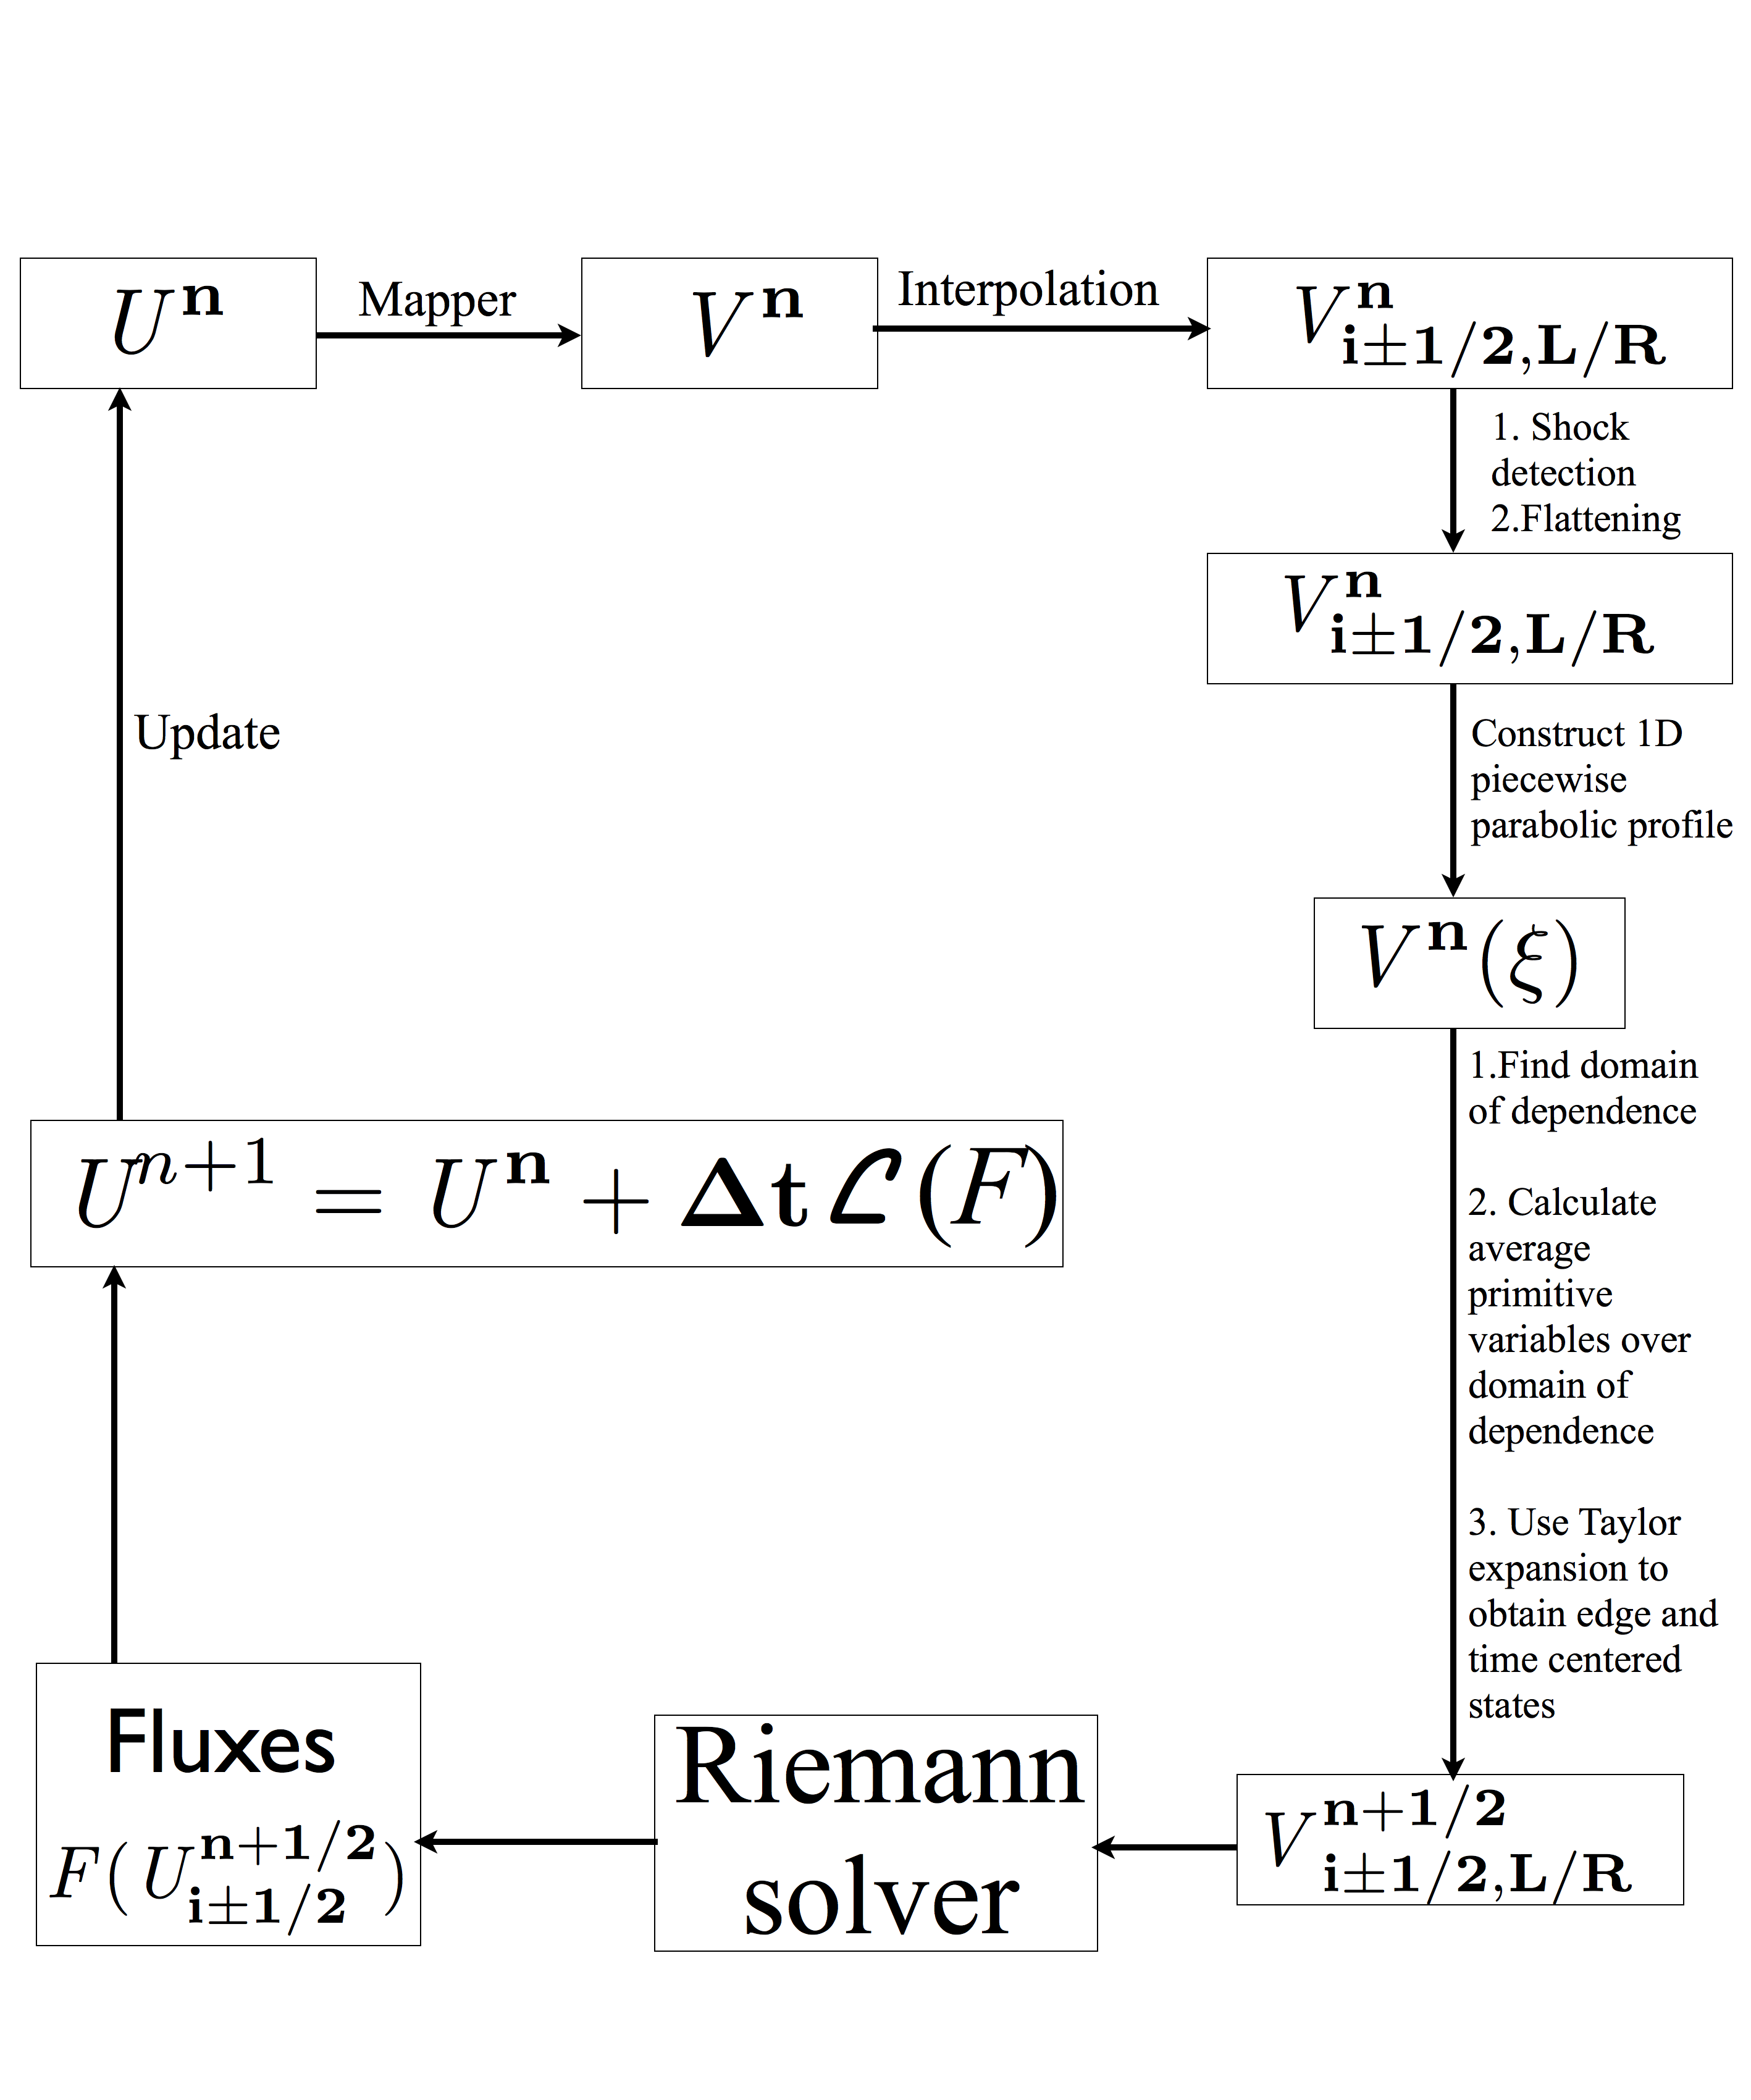
\includegraphics[width=\textwidth]{pfc.png}
%\caption{A flow diagram of the steps used in PLUTO for the numerical integration of the conservation laws. Here $U^n$, $V^n$, $F$, $\xi$, $\textmyfont{L}$ and $\Delta t$ are conservative variables, primitive variables, fluxes, volume coordinates, one-dimensional flux difference operator and the time step respectively. The index $n$ and the subscript $i\pm 1/2$ denote the time and location respectively. $L/R$ represent the left or right state. For example, $V^n_{i+1/2, L}$ is the value of primitive variables at time $t^n$ and left state at the cell interface $i+1/2$. Three main steps are used for the integration 1. the reconstruction: from the input $U^n$ estimate the cell edge state at half time step $U^{n+1/2}_{i\pm1/2, L/R}$, 2. the Riemann solver: estimates fluxes $F(U^{n+1/2}_{i\pm1/2})$ at the cell interfaces, 3. Update: estimate cell averages of coservative variables for the next time step $U^{n+1}$ and update them.}
%\label{f:pfc}
%\end{figure}

%Let $U^n$ and $U^{n+1}$ be the cell averages of the conservative variables over the i-th cell and time $t^n$ and $t^{n+1}$ respectively, $F\left (U_{i+1/2}^n\right )$ and $F\left ( U_{i-1/2}^n \right )$ the fluxes at the cell interfaces $i+1/2$ and $i-1/2$ respectively, $\Delta t=t^{n+1}-t^{n}$ the time-step and $\Delta x$ the cell width, then the basic Godunov scheme is given by
%\begin{equation}
%U^{n+1}= U^n - \frac{\Delta t}{\Delta x}\left [F\left (U^n_{i+1/2} \right )-F\left (U^n_{i-1/2} \right ) \right ].
%\end{equation}
%


PLUTO solves the system of conservation equations (\ref{eq:d}-\ref{eq:e}) using a finite volume formalism based on Godunov-type schemes. It performs the numerical integration of the fluid equations in three major steps: (1) Reconstruction, (2) Evolution of fluxes and (3) Update cell averages. 

%Fig.~\ref{f:pfc} shows a flow diagram of the steps used in PLUTO. In the following I discuss the steps shown in this figure. 
 
Prior to the reconstruction the conservative variables are transformed to primitive quantities. This transformation is required because primitive variables are used to solve the Riemann problem. In PLUTO, a mappers routine performs the transformation between the conservative and primitive variables. 
 
%%%%%%%%%%%%%%%%%%%% %%%%%%%%%%%%%%%%%%%%
%						Reconstruction
%%%%%%%%%%%%%%%%%%%%%%%%%%%%%%%%%%%%%%%%
\subsection{Reconstruction}
This is the first stage of computation where piecewise polynomial approximations to the primitives are estimated from the cell averages. In my models, I use the piecewise parabolic method available in PLUTO \citep{mignone05} to reconstruct the states at the cell interfaces. 
%This is the first stage of computation where the left and right states at the cell interfaces are estimated. The input cell averages of the conservative variables $U^n$ are first mapped onto primitive variables $V^n$ by a mapper routine. An interpolation routine is used to obtain the cell averages of the primitive variables at the cell boundaries $V^n_{i+1/2, L}, \ V^n_{i+1/2, R}, \ V^n_{i-1/2, L}, \ V^n_{i-1/2, R}$ (in compact form ($V^n_{i\pm1/2, L/R}$). A shock detection algorithm is used to scan the computation domain for strong shocks. At the shock location the interface states are modified by a flattening algorithm in order to prevent spurious oscillations. 

%A one-dimensional piecewise parabolic profile $V^n\left ({\xi} \right )$ (where $\xi$ is the generalised volume coordinates) is used to obtain values of the states inside each cell i. At each interfaces, the domain of dependence for each characteristic of the fluid is determined. The average of the primitive variables over the domain of influence is estimated using the piecewise parabolic profile. Then using a Taylor expansion the edge and time centred states $V^{n+1/2}_{i\pm1/2, L/R}$ are computed. 
%Finally a mapper routine calculate the edge and time centred conservative states $U^{n+1/2}_{i\pm1/2, L/R}$ from the corresponding primitive states.

 

%%%%%%%%%%%%%%%%%%%%%%%%
% 		Riemann solver
%%%%%%%%%%%%%%%%%%%%%%%%
\subsection{Estimation of fluxes}
 In this step, a suitable Riemann solver is used to estimate the fluxes at the cell boundaries. The input data for the Riemann solver are the left and right cell-edge states obtained from the reconstruction. 
% The input data for the Riemann solver are the left and right cell-edge states $V^{n+1/2}_{i\pm1/2, L}$, $V^{n+1/2}_{i\pm1/2, R}$ obtained from the reconstruction.
%\begin{equation}
%F_{\pm} = \textmyfont{R}(V^{n+1/2}_{i\pm1/2, L}, V^{n+1/2}_{i\pm1/2, R})
%\end{equation}

%A Riemann problem with an initial value,
%\begin{equation}
%V(x, 0) = \begin{cases}
%V_{i+1/2, L} \ \textrm{if} \  x < x_+,  \\
%V_{i+1/2, R} \ \textrm{if} \  x > x_+
%\end{cases}
%\label{eq:Rp}
%\end{equation}
%gives four different solutions depending on the initial values of the pressure on each side of the discontinuity: 1. a contact discontinuity separated by a shock and a rarefaction, 2. a contact discontinuity separated by two rarefactions, 3. a vacuum separated by two rarefactions and 4. a contact discontinuity separated by two shocks. All the above solutions are self-similar, which means  that the solutions can be expressed as a function of $x/t$. 
%
%The normal velocity and the pressure of the fluid are continuous across the contact discontinuity. However, across the shock  all the states have discontinuities. In the case of non-relativistic fluid, the tangential component of the velocity across the shock is continuous. However, in the case of relativistic fluid it may be discontinuous \citep{mignone07}. The discontinuities or, jumps of the states $[q]$ where  $q$ and $q_s$ are the pre and post shock states are described by Rankine-Hugoniot jump conditions.
%
%Let $v_1$ be the normal velocity, $v_2$ and $v_3$ the transverse velocity components, $v_{sh}$ the shock velocity, $\Gamma_{sh} = 1/\sqrt{1-v_{sh}^2}$ the Lorentz factor of the shock, and $j$ the mass flux across the shock.  Then the Rankine-Hugoniot jump conditions are given by:
%\begin{eqnarray}
%\left[\frac{1}{D}\right] = - \frac{\Gamma_{sh}}{j} [v_1] \label{eq:j1}\\
%\left[ h \Gamma v_1 \right ] = \frac{\Gamma_{sh}}{j}[p] \label{eq:j2}\\
%\left[ h \Gamma v_2 \right ] = 0 \label{eq:j3}\\
%\left[ h \Gamma v_3 \right ] = 0 \label{eq:j4}\\
%\left[ h \Gamma -\frac{p}{D} \right ]=  \frac{\Gamma_{sh}}{j} [pv_1] \label{eq:j5}
%\end{eqnarray}
%
%These equations of the jump conditions (Eq.~\ref{eq:j1}-\ref{eq:j5}) together with the enthalpy equation (Eq.~\ref{eq:enth}) are then solved to obtain the fluxes at the cell interfaces.
 
Among several Riemann solvers that PLUTO provides, I use the least diffusive two shock Riemann solver \citep{mignone05} for the axisymmetric models (presented in chapters \ref{chapter4}, \ref{chapter5}, \ref{chapter6} and \ref{chapter7}). This solver solves Riemann problems at each zone by approximating rarefaction waves as shocks. 
At locations of shocks the two-shock solver is switched to a more diffusive HLL solver to avoid artificial oscillations.

For the three dimensional precessing jet model (presented in chapter~\ref{chapter8}) I used the HLL Riemann solver. 





%%%%%%%%%%%%%%%%%%%%%%%%
%		Update cell averages
%%%%%%%%%%%%%%%%%%%%%%%%
\subsection{Update cell averages}

In the final step, the fluxes at the cell boundaries are used to estimate the cell averages of the states of the next time step utilising a time marching scheme. 

%Let the volume average of the initial conservative variables $\bar{U}^n$ are given as: 
%\begin{equation}
%\bar{U}^n = \frac{1}{\Delta \textmyfont{V}}\int U d\textmyfont{V}
%\end{equation}
%where $\Delta\textmyfont{ V}$ is the control volume. 

%where d = 1, 2, 3 indicates the direction. 
% 
%
%The one dimensional flux differencing operator $\textmyfont{L}^d$ is given by,
%\begin{equation}
%%\textmyfont{L}^d = - \frac{\Delta t}{\Delta \textmyfont{V} }\left[F^d(U_{\textmyfont{x}+1/2}^{n+1/2})A^d_{\textmyfont{x}-1/2}-F^d(U_{\textmyfont{x}-1/2}^{n+1/2}) A^d_{\textmyfont{x}-1/2}\right ]
%\textmyfont{L}^d = - \frac{1}{\Delta \textmyfont{V}^{\ d}}\left ( A_+^d\textbf{F}_+^d - A_-^d\textbf{F}_-^d\right ) + \textbf{S}^d
%\label{ea:up}
%\end{equation}
%where $A_{\pm}^d$ is the area of the cell interfaces and $\Delta \textmyfont{V}^{\ d}$ is the volume along the direction d. These two quantities $A_{\pm}^d$ and $\Delta \textmyfont{V}^{\ d}$ depend on the geometry used for the model (see Table 1 of \citep{mignone07} for values of $A^d$ and $\Delta \textmyfont{V}^{\ d}$ in different coordinate systems). The suffix $\pm$ represents $i\pm1/2$, $j\pm1/2$, $k\pm1/2$ when $d$ = 1, 2 and 3 respectively.  
%
%The flux can be estimated either by using Strang operator splitting method or simultaneous estimation in all directions. 

Among the time-marching schemes provided by PLUTO, I used the characteristic tracing scheme with i) A directionally split method to solve the two dimensional models  ii) A dimensional unspilt method to solve the three dimensional models. A directionally split method is computationally least expensive, since it solves $n$ Riemann problems for an $n$-dimensional problem. On the other hand, a directionally unsplit method utilises the corner transport upwind method \citep{colella90} and is computationally expensive because it solves more Riemann problems. With a directionally unsplit method in two and three dimensional problems, solutions for 4 and 12 Riemann problems are required (in stead of 2 and 3). However, directionally unspoilt methods are preferable to directionally split methods because they avoid errors resulting from operator splitting. 
% it is preferred over dimensionally split method because it avoids errors due to operator splitting.      
%In my models I use the dimensional splitting scheme while for the time marching I use the Characteristic tracing method. 

The time step $\Delta t$ is restricted by the Courant-Friedrichs-Lewy (CFL) condition;  
%\begin{equation}
%\Delta t = \left ( \frac{\Delta l_{\rm min}}{\lambda_{\rm max}^d}\right )
%\end{equation}
% where $\Delta l_{\rm min}$ is the smallest cell length and $\lambda_{\rm max}^d$ is the largest signal velocity in the direction r. 
I used CFL = 0.4 and 0.2 for the cases of two and three dimensional models respectively. 

\subsection{Shock capturing}
%For the combination of dimensional splitting and characteristic tracing schemes, $n$ Riemann problems are required to be solved in each direction for a $n$-dimensional model. The estimated fluxes from the Riemann solver are then used in Eqn.~\ref{eq:upd} to obtain the temporal update of the cell averages.  
%(see \citep{mignone05} for the details of two shock Riemann solver)
\begin{figure}[h!]
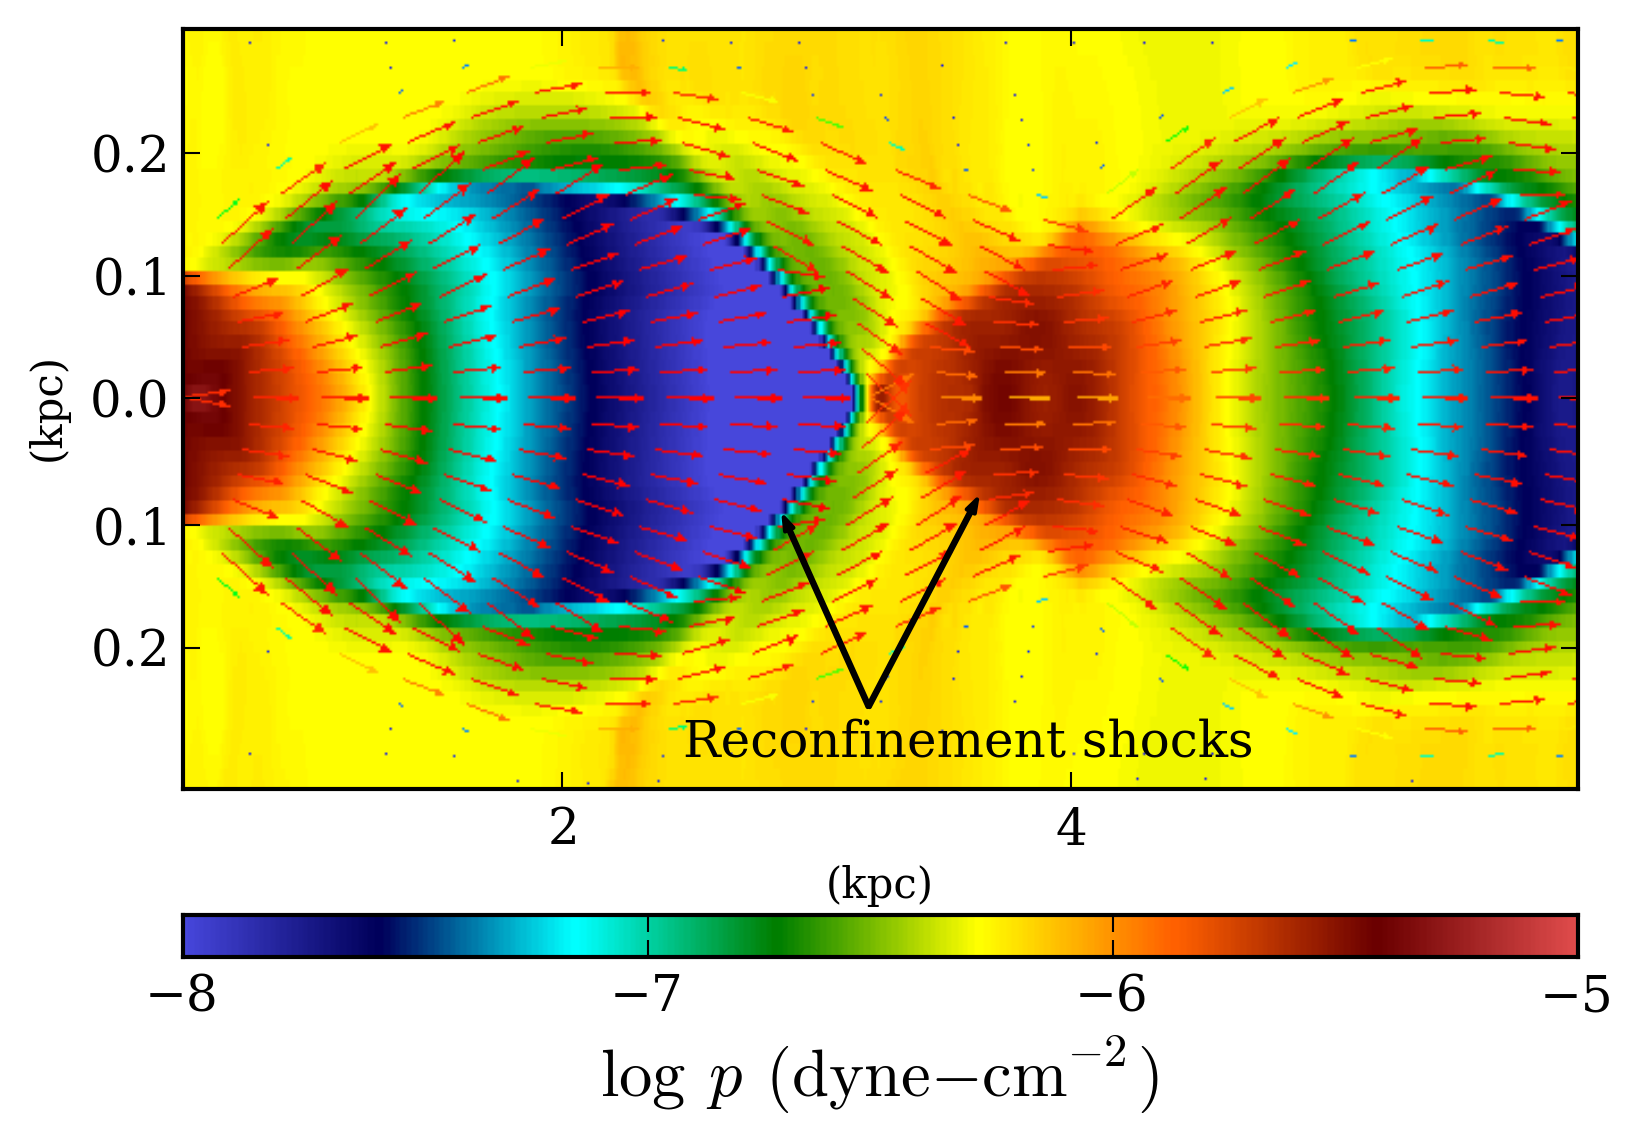
\includegraphics{rsk.png}
\caption{Inner 6~kpc of one of my two dimensional axisymmetric jet-ICM interaction models (model Civ with $r_{\rm}=0.1$~kpc, $p_{\rm jet}/p_{\rm a}$, $\beta=0.8$, $\chi = 12.75$). This pressure image shows the ability of the PLUTO to capture the Reconfinment shocks. The arrows represents the flow direction. }
\label{f:rsk}
\end{figure}

PLUTO is an excellent hydrodynamic code for capturing shocks. Fig.~\ref{f:rsk} shows the inner 6~kpc of one of my two dimensional jet-ICM interaction model solved by PLUTO (model Civ of chapter~\ref{chapter5} with jet inlet radius $r_{\rm}=0.1$~kpc, overpressure ratio $p_{\rm jet}/p_{\rm a}$ = 5, jet velocity in units of the speed of light $\beta=0.8$, and jet density parameter $\chi = 12.75$). In this pressure image (overlaid with the flow vectors), we see the reconfinement shocks (marked by black arrows) are well captured. This is an illustration of the performance of PLUTO in shock capturing.  

%%%%%%%%%%%%%%%%%%%%%%%%%%%%%%
%		Test parallel computing performance
%%%%%%%%%%%%%%%%%%%%%%%%%%%%%%
\section{Scaling of PLUTO code}\label{s:pt}
\begin{figure*}
\centering
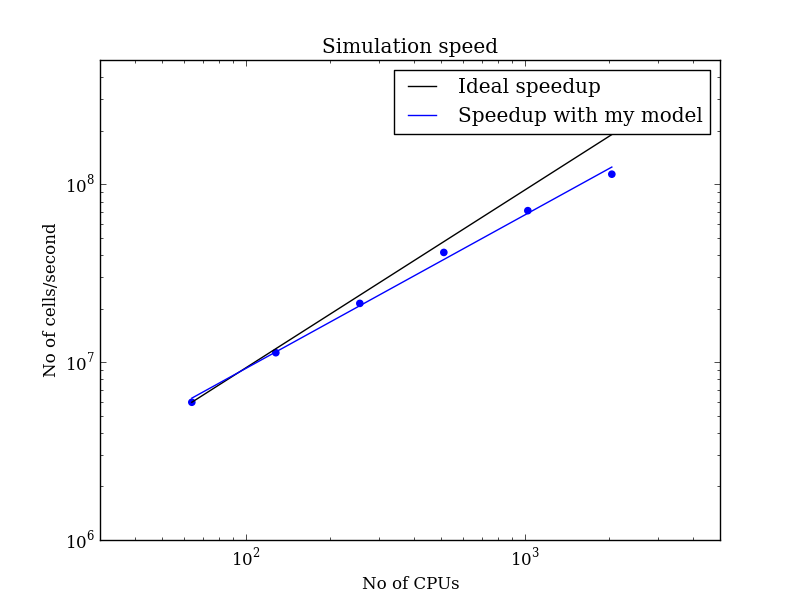
\includegraphics[width=12cm]{ppt.png}
\caption{ The points represent the computed number of cells per second (wall clock) for my three dimensional jet-ICM interaction model. A power law fit to the points with a power law index 0.86 is shown by a blue line. For a comparison an ideal speedup of a code is also shown (black line). }
\label{f:ppt}
\end{figure*}

\begin{table*}
%\begin{sidewaystable}[htbf]
\caption{Scaling test for PLUTO.}
\centering
\begin{tabular}{l * {3}{c}}
\hline \hline
No. of CPU & average time/step (s) & Cells/sec & Cells/sec/cpu  \\
\hline 
    %%%%%%%%%% 		Medium resolution	%%%%%%%%%%%%%%%
	%\multicolumn{4}{c}{Medium resolution model (256 $\times$ 256 $\times$ 256)} \\ 
	%\hline
	 64   & 2.82  &  3.57$\times10^6$ &   5.58$\times10^4$    \\
	 128 & 1.48  & 6.82$\times10^6$ &  5.32$\times10^4$ \\
	 256  & 7.85$\times10^{-1}$ & 1.28$\times10^7$  & 5.00$\times10^4$ \\
	 512  & 4.05$\times10^{-1}$ & 2.49$\times10^7$  & 4.86$\times10^4$ \\
	 1024 & 2.36$\times10^{-1}$ & 4.27$\times10^7$  & 4.17$\times10^4$ \\
	 2048  & 1.47$\times10^{-1}$ & 6.86$\times10^7$  & 3.35$\times10^4$ \\
	\hline
	  %%%%%%%%%% 	High resolution	%%%%%%%%%%%%%%%
\end{tabular}
\label{t:pst}
%\end{sidewaystable}
\end{table*}

%	\multicolumn{3}{c}{High resolution model (456 $\times$ 456 $\times$ 456)} \\ 
%	\hline
%        512    &  2.49$\times10^7$  & 4.86$\times10^4$  \\
%        1024  &  3.72$\times10^7$  & 3.63$\times10^4$ \\
%        2048  & 7.65$\times10^7$  & 3.74$\times10^4$ \\
%	 \hline

I performed a scaling test for the PLUTO code using my three dimensional jet-ICM interaction model (resolution = $256^3$) with different numbers of CPUs. I ran a three dimensional model (run A of chapter~\ref{chapter7}) for a fixed wall clock time = 300 sec with 64, 128, 256, 512, 1048 and 2056 cpus and record the average time (wall clock) required for a step, the computed number of cells per second (wall clock), and the computed number of cells per sec (wall clock) per cpu ( see Table.~\ref{t:pst}). Fig.~\ref{f:ppt} shows the number of cells computed per second (vertical axis) for different numbers of processors (horizontal axis). Fitting a power law to the points shown in Fig.~\ref{f:ppt} I obtained a power law index 0.86, which indicates a nearly linear speed up of the code. For a comparison the ideal speedup of the code is shown by a black line (power law index = 1). 

% power law index=1 implies a linear speedup of the algorithm. Linear Speedup: In which case double the number of cells increase the computation speed twice. 


%%%%%%%%%%%%%%%%%%%%%%%%%%%%%%
%			Problem initialisation and BC
%%%%%%%%%%%%%%%%%%%%%%%%%%%%%%
\section{Problem initialisation for the simulations in this thesis}
\begin{figure*}
\centering
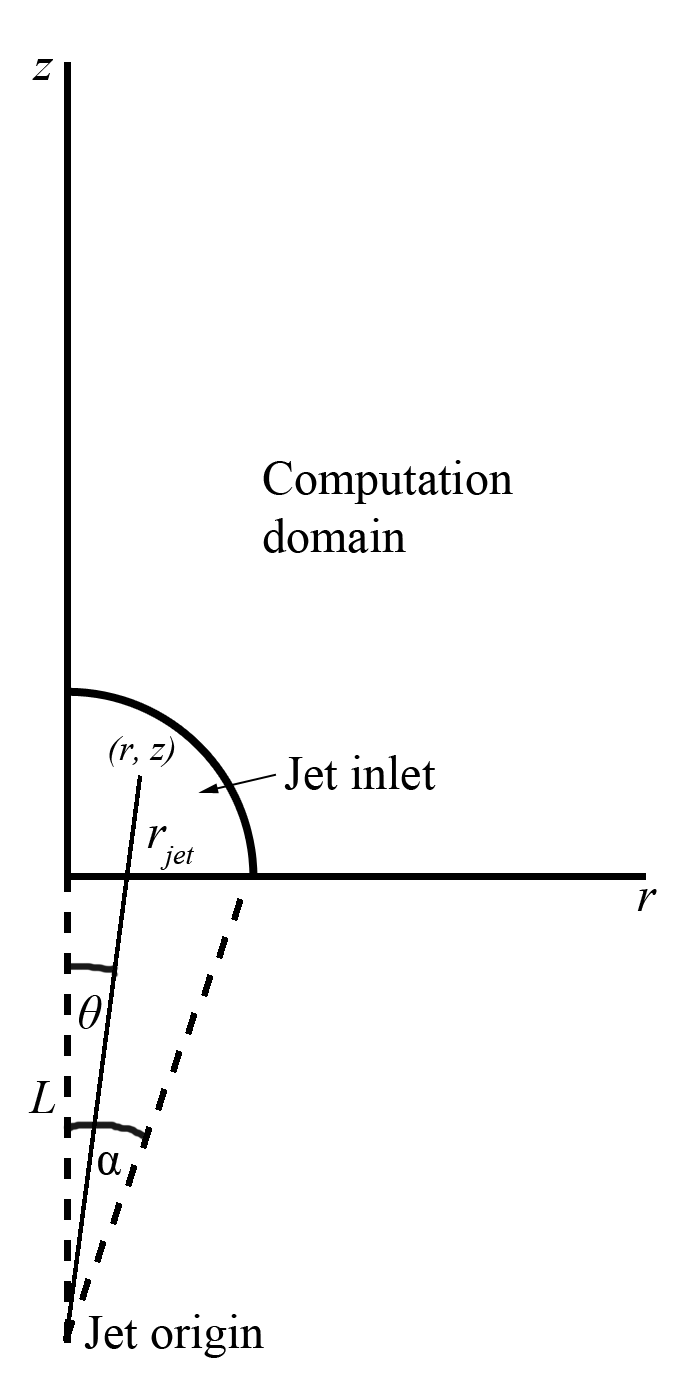
\includegraphics[width=5cm]{cjt.png}
\caption{Schematic diagram of the initialisation of a conical jet (marked by dashed lines) with half cone angle $\alpha$ into the ($r, z$) computation domain. An initial quarter circular jet inlet with radius $r_{\rm jet}$ is used to initialise the jet in the computation domain. This initial jet inlet is useful to avoid reverse shocks running across the ghost zones. The velocity components inside the jet inlet are: $v_r = r/\sqrt{(L+z)^2+r^2}$ and $v_z = (L+z)/\sqrt{(L+z)^2+r^2}$. }
\label{f:cjt}
\end{figure*}

%As I discussed in the chapter~\ref{introduction} the main goal of the thesis is to study the key features of the inner 10~kpc of the northern jet of Hydra A. My initial assumption is that the two bright knots in the northern jet within 10~kpc is the reconfinement shocks produced by the interation of the over pressured jet with the environment.  

The main aim of this thesis is to study the key features of the inner 20~kpc on the northern side of Hydra A. I perform my study in two stages- i) First, model the inner 10~kpc of the northern jet using an axisymmetric model and obtain best fit jet parameters; ii) Second, utilising the best fit jet parameters model the inner 20~kpc with a three dimensional precessing jet model. 

\subsection{Axisymmetric model}
The main focus of this study is the bright knots within the central 10~kpc of the northern jet. As I discussed in chapter~\ref{introduction}, these bright knots are considered as reconfinement shocks. In the numerical study of AGN jets, the jet can be considered as either initially parallel \citep{sutherland07} or initially conical \citep{komissarov98, krause12}. In both cases, jets are recollimated by reconfinement shocks. However, considering the fact that the jets emerge from the central black and initially expands in the environment (analyzing VLBI pc scale \citep{taylor96} and VLA kpc scale \citep{taylor90} data of Hydra A, I find that the jet expands by a factor of approximately 200 between the parsec scale and the kilo parsec scale), the initially conical jet model is more realistic. Therefore, I use an initially conical jet model such as used by \citet{komissarov98}. 

%effects of the jet-ambient medium interaction, for example, the mass or energy transport by the jet, it is not important whether the jet is initially parallel or conical. However, structures such as reconfinement shocks along the jet axis, are sensitive to the initial jet radius and the opening angle of the jet. Moreover, the fact that AGN jets are emitted from the black hole implies that they are initially expanding. For instance, the VLBI pc scale data (Taylor, 1996) and VLA kpc scale data (Taylor et al., 1990) of the Hydra A indicate that the jets expand from approximately 1 pc to approximately 200 pc. Therefore, for the modelling of jet structures near the core, a conical opening jet is more realistic. In the models presented in this chapter I use initially conical jet model following Komissarov & Falle (1998).

%\noteM{(Analyzing the data of VLBI pc scale \citep{taylor96} and VLA kpc scale \citep{taylor90} jets of Hydra A I obtain that the jet is initially freely expanding)}

The $(r, z)$ computational domain for the axisymmetric simulations is a cylinder of radius $r=25$ kpc and height $z=50$ kpc. The conical jet marked by dashed lines in Fig.~\ref{f:cjt} with a half cone angle $\alpha$, enters into the computation domain at a distance $L=0.5$~kpc away from its origin. To initialise the jet in the computation domain, I use a quarter circular jet inlet with radius $r_{\rm jet}$. The velocity components inside the jet inlet are:
\begin{eqnarray}
v_r = vr/\sqrt{(L+z)^2+r^2} \\
v_z = v(L+z)/\sqrt{(L+z)^2+r^2}
\end{eqnarray} 
where $v=\sqrt{{v_r}^2+v_z^2}$ is the magnitude of the jet velocity. The other component of the velocity $v_\theta$ is initially set at 0. The initial quarter-circular jet inlet in the computation box prevents reverse shocks running through the ghost zones. 
The jet power is fixed for all models $P_{\rm jet} = 10^{45} $~erg s$^{-1}$. The estimation of jet power is described in Chapter~\ref{chapter3}. Analysing the pressure of the VLBI jet of Hydra A \citep{taylor96} and the X-ray atmosphere pressure \citep{david01} I choose initial jet overpressure ratio 2 and 5. Based on the data provided for the full width half maximum (FWHM) of the northern Hydra A jet \citep{taylor90}, the jet inlet radius is chosen to between 80 and 180~pc. The jet velocity $\beta$ (in unit of the speed of light) is a free parameter and is chosen in the range 0.4-0.95. The remaining jet parameter, the density parameter $\chi$ (defined in Chapter~\ref{introduction}) is determined by the other parameters according to the relationship among relativistic jet parameters provided by \citep{sutherland07} (see \S~\ref{s:model} for details of the model). For each model with different jet parameters I record data for the jet boundary and the locations of the reconfinement shocks. Fitting both of these simulated jet boundary and the shock location with the observed jet boundary and bright knots locations I estimate a theoretical velocity for the northern Hydra A jet. This procedure is explained in Chapter~\ref{chapter5}.

A tracer $\tau$ for the jet is used to track the jet plasma in the various regions of the computation domain. The tracer obeys an advection law of the form: 
\begin{equation}
\frac{\partial \rho \tau}{\partial t}+ \nabla \cdot (\rho \tau \textbf{v}) = 0
\end{equation}

%I use the \citet{taub1948a} equation of state, a quadratic approximation to the exact Synge--J\"{u}ttner relativistic perfect gas equation of state \citep{juttner1911a,synge1957a}, which yields $\gamma\rightarrow5/3$ in the low temperature limit, and $\gamma\rightarrow4/3$ in the high temperature limit. 

Because the radiative cooling time of the ambient gas and the synchrotron cooling time of the jet plasma are both large compared to the simulation time (which is equivalent to the jet crossing time), I do not include radiative cooling in the simulations.

The cluster environment is constructed using analytical fits for the density, pressure and temperature data derived from the X-ray data presented by \citet{david01} (see chapter~\ref{chapter3} for details).

\subsection{Precessing jet model}
\begin{figure}
\centering
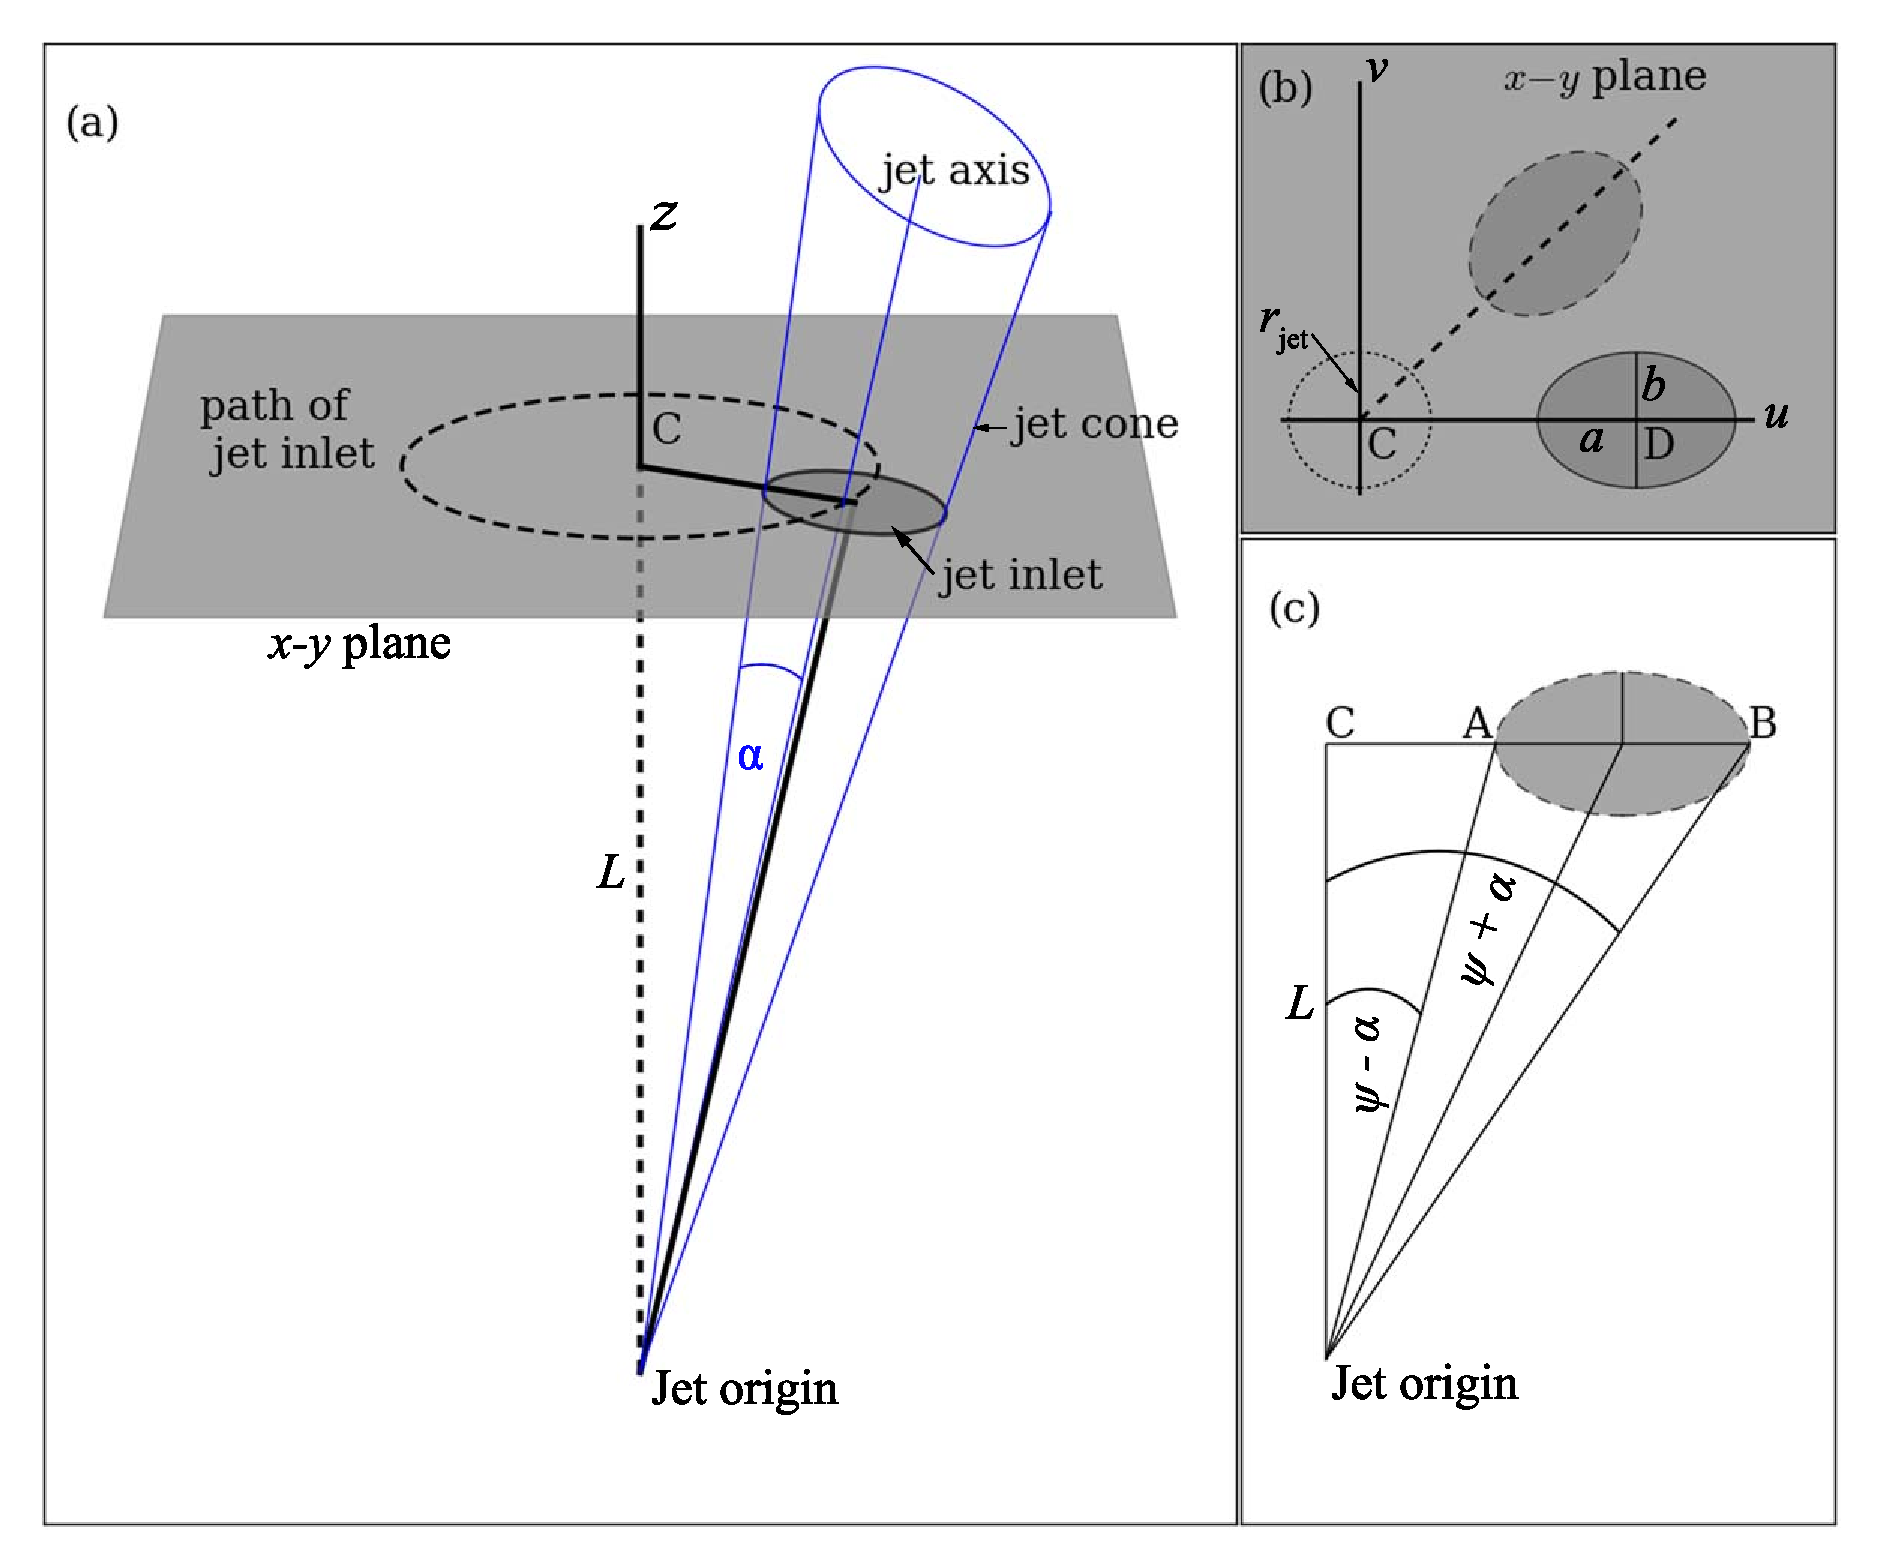
\includegraphics[width=\linewidth]{fig2.eps}
\caption{Geometry of the precessing jet model. Panel (a) shows  the conical jet originating at a distance $L$ below the $x-y$~plane of the computational domain. The precessing jet cone intersects the $x-y$~plane in an elliptical jet inlet which moves on the (dashed) circular path. The coordinates $(u,v)$, defined by the intersection of the cone and the $x-y$~plane at a precession azimuth $\phi = 0^{\circ}$ and an arbitrary $\phi$ are shown in panel (b). The dotted circular line is the intersection of the cone when the precession angle $\psi = 0^{\circ}$.
The jet semi-minor axis of the jet inlet $b$ is equal to the jet radius $r_{\rm jet}$.  In panel (c) the angles defined by the lines joining the jet origin and the left and right edges of the inlet ellipse are shown. These define the semi-major axis of the ellipse.}
\label{f:mod}
\end{figure}
The main focus of this part of my thesis is the curvature of the jet and the jet to plume transition on the northern side of Hydra A. As I discussed in chapter~\ref{introduction}, the complex morphology of the Hydra A jets is a result of a dynamical interaction between precessing jets and the intracluster medium (see chapter~\ref{chapter6} for details of the model).

 The geometrical configuration of the precessing jet model for the Hydra A northern jet is shown in Fig.~\ref{f:mod}.  The jet originates near the central black hole (marked as the jet origin in panel (a)) and is initially ballistic and conically expanding \citep{komissarov98, krause12, nawaz14a}. It precesses around the $z$-axis with a precession period $P$ and a precession angle $\psi$. The best fit axisymmetric model (see chapter~\ref{chapter5}) gives a jet radius $r_{\rm jet} = 0.1$~kpc at a distance $L=0.5$~kpc from the black hole. The half cone angle of the jet cone is then $\alpha = \tan^{-1}(r_{\rm jet}/L) = 11.3^{\circ}$.

The jet cone intersects the $xy$~plane at a distance $L$ from the central black hole in an ellipse. As a result of precession the elliptical jet inlet follows a circular path (marked in panel (a)) on the $xy$~plane. The elliptical jet base is determined from the geometry shown in panels (b) and (c) of Fig.~\ref{f:mod} as described below.  

Let $(u,v)$ be a rotating frame fixed on the elliptical jet inlet. The semi-major axis $a$ and semi-minor axis $b$ of the ellipse lie on the $u$ and $v$ axes respectively (see panel (b) of Fig.~\ref{f:mod}). The centre of the ellipse lies at 
\begin{eqnarray}
u_0 = L[\tan(\psi+\alpha) - \tan(\psi - \alpha)]/2, \\
v_0 = 0.
\end{eqnarray}
%GVB
%From the geometry of panel (b) and (c) we obtain 
From the geometry described in panels (b) and (c) we obtain 
\begin{eqnarray}
a &=& L[\tan(\psi + \alpha) - \tan(\psi -\alpha)]/2, \\
b &=& r_{\rm jet}.
\end{eqnarray}
Therefore, in the rotating $(u,v)$ coordinate system the jet inlet is defined by 
\begin{equation}
(u - u_0^2)/a^2 + v^2/ b^2 \leq 1.
\end{equation}
For a counter-clockwise rotation of the jet inlet the coordinates $uv$ are related to the computational coordinates $xy$: 

\begin{eqnarray}
u &=& x\cos \phi + y \sin \phi, \\
v &= &- x \sin \phi + y \cos \phi,
\end{eqnarray} 
%aln
here $\phi = 2\pi t/P$ is the azimuth angle of the precession. 

In order to avoid reverse shocks running through the ghost zones I initialise the jet in the computational domain with a semi-ellipsoidal cap above the jet inlet with semi-principle axes $a, \ b$ and $c (= a)$. 

%The input jet parameters, the jet kinetic power $P_{\rm jet} = 1\times 10^{45}$~erg s$^{-1}$, the jet over-pressure ratio $p_{\rm jet}/p_{\rm a} = 5$, the jet velocity $\beta = 0.8$, and the jet density parameter $\chi = 12.75$ are chosen from the best fit axisymmetric model presented in Paper I. We explore a range of values for the precession period $P = 1, 5, 10, 15, 20, 25$~Myr and the precession angle $\theta = 15^{\circ} \rm \ and \ 20^{\circ}$. The grid of models is presented in Table~\ref{t:mod}. Since the radiative cooling time of the environment is large compared to the simulation time, we do not include cooling in our models. 

As described in the axisymmetric model, the three-dimensional cluster environment is constructed using analytical fits for the density, pressure and temperature data derived from the X-ray data published by \citet{david01}.
 
%I set up the computational grid as follows. I use a high resolution $156^3$ uniform grid for the inner 5~kpc$^3$, thereby resolving the jet base by six cells. For the remaining computational domain I use stretched grid with 100 additional cells along each of the coordinate directions. 

%The simulations were performed with the publicly available relativistic hydrodynamic code PLUTO \citep{mignone07}, which solves the relativistic gas dynamical equations using the finite volume method based on Godunov type schemes. 



\subsection{Grid}
\paragraph{Axisymmetric model:}
\begin{figure*}
\centering
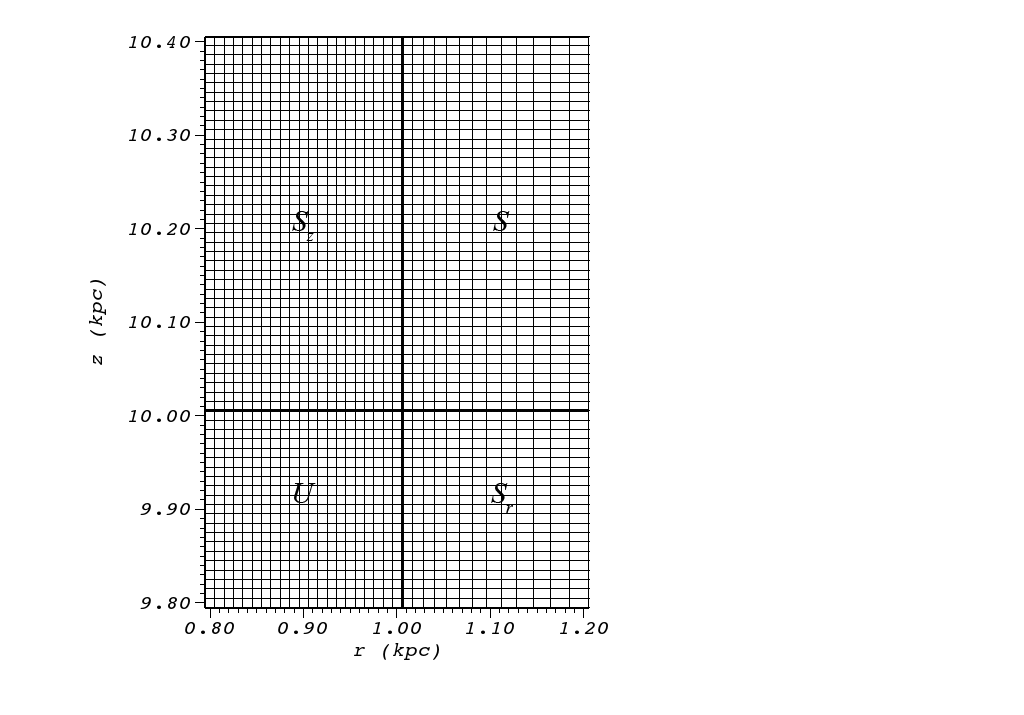
\includegraphics[width=\linewidth]{sgr.png}
\caption{A small segment of the computation domain ($r= 0.8 - 1.2~ \rm kpc, z = 9.8-10.4~\rm kpc$) of an axisymmetric model (run cv of chapter~\ref{chapter5}) at the intersection where the stretching ratios change in the $r$ and $z$ directions. The bold vertical and the bold horizontal lines are the boundaries of the uniform grid in $r$ and $z$ directions respectively. These two bold lines divide the computation domain into four differently resolved zones marked by $S_z, \ S, \ U,$ and $S_r$, i) $S_z$: uniform in  $r$ and stretched in $z$ direction, ii) $S$: stretched in both directions, iii) $U$: uniform in both directions, iv) $S_r$: stretched in $r$ direction and uniform in the $z$ direction. Since I focus the jet structures along its axis, I use less stretching in jet direction $z$.}
\label{f:sgr}
\end{figure*}

PLUTO provides two different grid structures- uniform grid and stretched grid. If $x_R$, and $x_L$ are the leftmost and rightmost points of the grid patch and N is the number of  points then a uniform grid is constructed with cell spacing $\Delta x$
\begin{equation}
\Delta x = \frac{x_R-x_L}{N}
\end{equation} 
Provided that a uniform grid patch is present, the grid can be stretched in any direction with a stretching ratio $s$ and maximum number of points N
\begin{equation}
\Delta x_i = \Delta x s^i
\end{equation}
where $i = 1, 2, ..., N$ indicates the cell position in the stretched grid, $\Delta x_i$ is the respective cell width and $\Delta x$ is the cell width of the closest uniform grid.
From the following relationship the stretching ratio is estimated using a Newton algorithm. 
\begin{equation}
s\frac{1-s^N}{1-s}= \frac{x_R-x_L}{\Delta x}
\end{equation}
where $x_L$ and $x_R$ are the leftmost and rightmost points. 

Using a combination of uniform and stretched grids described above I define a high resolution uniform grid within the central $1\,\mathrm{kpc}\times10\,\mathrm{kpc}$ region and a lower resolution streched grid in the outer region. The structures of the different grid patches are as follows: \\
\begin{itemize}
\item Uniform grid, $U$: In the inside 1$\times$10~kpc zone a uniform grid with 100$\times$1000 cells is used. The cell width for this grid patch is 0.01 kpc. 
\item Grid stretched in $r$, $S_r$: The grid patch in the domain 1 to 25~kpc in $r$ and 0 to 10~kpc in $z$ direction is stretched in the $r$ direction and uniform in the $z$ direction. 90 points are used to stretch the grid along $r$. The stretching ratio is 1.009.  
\item Grid stretched in $z$, $S_z$: The grid patch in the domain 0 to 1~kpc in $r$ and 10 to 50~kpc in $z$ direction is stretched in the $z$ and uniform in the $r$ direction. 400 points are used to stretch the grid along $z$. The stretching ratio is 1.055. 
\item Stretched grid, $S$: The grid patch in the domain 1 to 25~kpc in $r$ and 10 to 50~kpc in $z$ direction is stretched in both $r$ and $z$ direction.
\end{itemize}
Since I focus the structures of the Hydra A northern jet along its axis $z$, I choose less stretching along the jet direction.
 
 Fig.~\ref{f:sgr} shows a small segment ($r= 0.8 - 1.2~ \rm kpc, z = 9.8-10.4~\rm kpc$) of the computation domain. Here we see two bold lines, the bold vertical line (boundary of the uniform grid along $r$) and the bold horizontal line (boundary of the uniform grid along $z$) divide the computation domain into four zones marked by $S_z, \ S, \ U,$ and $S_r$: i) $S_z$: uniform in the $r$ and stretched in the $z$ direction, ii) $S$: stretched in both directions, iii) $U$: uniform in both directions, iv) $S_r$: stretched in the $r$ and uniform in the $z$ direction. 
 
 \paragraph{Precessing jet model:}
 For the 3D precessing jet model I set up the computational grid as follows. I use a high resolution $156^3$ uniform grid for the inner 5~kpc$^3$ ($-2.5 < x < 2.5$, $-2.5 < y < 2.5$, and $0.5 < z < 20.5$, where the units here are kpc ), thereby resolving the jet base by six cells. For the remaining computational domain I use a stretched grid with 100 additional cells along each of the coordinate directions. The stretching ratio along the $-x$, $x$, $-y$, and $y$ axes is 1.05 and the stretching ratio along the $z$-axis is 1.03. 

\subsection{Boundary conditions}
\paragraph{Axisymmetric model:}
I choose an axisymmetric boundary condition (available in PLUTO) for the boundary $r=0$ (axis of symmetry). For an axisymmetric boundary condition velocity components, $v'_r, \ v'_z \ \rm and v'_{\theta}$ and other states $q'$ (pressures or, density) in the ghost zones are:
\begin{eqnarray}
v'_r = -v_r  \\
v'_z = v_z \\
v'_{\theta} = -v_{\theta}  \\
q' = q
\end{eqnarray}
where $v_r, \ v_z, \ \rm and v_{\theta}$ are the velocity components in the computation domain. 

I impose a reflective boundary condition for $z=0.5$ by setting 
\begin{eqnarray}
v'_r = -v_r  \\
v'_z = v_z \\
v'_{\theta} = v_{\theta}  \\
q' = q
\end{eqnarray}

The remaining boundaries are chosen to be outflowing boundaries (available in PLUTO) satisfying the conditions: 
\begin{eqnarray}
\frac{\partial\textbf{v}}{\partial n}= 0 \\
\frac{\partial q}{\partial n}= 0
\end{eqnarray}
where $\textbf{v}$ is the velocity vector in the ghost zone and n is the coordinate direction orthogonal to the boundary. 

\paragraph{Precessing jet model:} 
I set up the boundary condition for the 3D precessing jet model as follows. I use a reflective boundary condition for the $z = 0.5$ plane by setting the velocity components in the ghost zones $v'_x$,  $v'_y$, $v'_z$ and other states $q'$ as 
\begin{eqnarray}
v'_x = v_x  \\
v'_y = v_y \\
v'_z = -v_z  \\
q' = q
\end{eqnarray}
where, $v_x$, $v_y$ and $v_z$ are the velocity components in the computation domain. 

For the remaining boundaries I choose outflowing boundary conditions. 

